\documentclass{sig-alternate-10pt}
\usepackage{graphicx}
%\usepackage{balance}
\usepackage{comment}
\usepackage{times,epsfig,subfigure,endnotes,color,url,paralist,multirow,float}
\usepackage{epstopdf}
\usepackage[pdftex]{hyperref}
%\hypersetup{
%	pdftitle={SIGCHI Conference Proceedings Format},
%	pdfauthor={LaTeX},
%	pdfkeywords={SIGCHI, proceedings, archival format},
%	bookmarksnumbered,
%	pdfstartview={FitH},
%	colorlinks,
%	citecolor=black,
%	filecolor=black,
%	linkcolor=black,
%	urlcolor=black,
	%breaklinks=true,
%}

\begin{document}

\title{IoT Middleware over Information-Centric Network}
\numberofauthors{1}
\author{
\alignauthor 
Sugang Li, Yanyong Zhang, Dipankar Raychadhuri\\
Ravi Ravindran, Qingji Zheng, Guoqiang Wang\\
\affaddr{WINLAB, Rutgers University, North Brunswick, NJ, USA}\\
\affaddr{Huawei Technologies, Santa Clara, CA,USA}\\
}
\maketitle
\begin{abstract}
Many approaches have been proposed to build a unified IoT platform where physical and digital objects are accessible by applications crossing different organization and domains, and are based on IP-overlay architecture.
%To build a unified IoT platform in which physical and digital objects can be accessible by application across different organization and domain, many state of art approaches are based on IP-overlay architecture.
These solutions inherit the constraints of the current internet, especially in terms of naming, heterogeneity, mobility and security.
In this paper, we propose a new Information-Centric Network (ICN) based IoT middleware to address these challenges by leveraging various promising features of ICN, such as naming. We elaborate the functions of ICN-based IoT middleware by integrating with the two future internet architectures, namely Named-Data Networking and MobilityFirst. Moreover, we evaluate the efficiency of service discovery (one of the functions in the proposed ICN-based IoT middleware) and demonstrate the feasibility of the proposed ICN-based IoT middleware .
%Thus, we propose a new Information-Centric Network (ICN) based IoT middleware to address these challenges. In this paper, we introduce detailed protocol design for the functions in the middleware, and evaluate the efficiency of service discovery.
\end{abstract}

\section{Introduction}
Many standalone Internet of Things (IoT) platforms have been developed and deployed in different domains in the past. The recent trend, however, is to evolve towards a globally unified IoT platform, in which billions of objects can connect to the Internet, interact with each other and inter-operate with many different applications  across the boundaries of organization and domains.

%in which billions of objects connect to the Internet, available for interactions among themselves, as well as interactions with many different applications across boundaries of administration and domains.

Building a unified IoT platform, however, poses a set of unique challenges and requirements on the underlying network and systems.
\begin{itemize}
\vspace{1mm}\item{\bf Identity}:
To realize a unified IoT platform, the first step is
%the capability
to assign names (or IDs) that are unique and unified within the scope and lifetime of each device, data items generated by these devices, or a group of devices towards a common objective. Currently, IoT systems have multiple vertical stacks with their own identity mechanisms that do not inter-operate with one another.

\vspace{1mm}\item{\bf Heterogeneity}:
IoT devices will have heterogeneous means of connecting to its application environment, and often have resource constraints, e.g., constrained resources in power, computing, storage and bandwidth.

\vspace{1mm}\item{\bf Mobility}:
In some scenarios, the data producer is mobile and unable to provide reliable connection with data consumers. Thus, in presence of mobility, a unified IoT platform requires the system to deliver IoT data within delays that are acceptable to applications.

\vspace{1mm}\item{\bf Security}:
The heterogeneity and openness of the IoT environment imposes great attack surface towards IoT devices and services. Without carefully considering security concerns such as identity authentication, data integrity and privacy, any IoT platform is hard to be adopted by either end-users or enterprises.
\end{itemize}

%Firstly, it needs to support a large number of networked objects - Cisco predicts there will be around 50 Billion IoT devices (sensors, RFID tags, actuators, etc) on the Internet by 2020 ~\cite{ciscovisual}and many of these objects are mobile, for smoothly with respect to metrics like response time, throughput, resolution and routing scalability. Secondly, IoT devices will have heterogeneous means of connecting to the Internet, and often have severe resource constraints, e.g., constrained resources in power, computing, storage, bandwidth. Thirdly, interactions between the applications and objects are often private, contextual, real-time and dynamic, requiring strong security and privacy  protections.
\subsection{ICN-IoT Middleware}
Current approaches towards a unified IoT platform are mostly based upon Internet overlays, whose inherent inefficiencies hinder the platform from satisfying the challenges outlined earlier. In recent years, in order to address  the inefficiencies of today's Internet, Information-Centric Network (ICN) has been proposed. ICN identifies a network object (including a mobile device, content, or service) by an application-centric name instead of its IP address, and adopts the name-based routing
%, lending itself to supporting the unified IoT platform.
In this paper, we propose a unified IoT middleware, referred to as \emph{ICN-IoT} middleware, which can support several specific ICN architectures. As shown in Figure~\ref{fig:mid_arch}, the ICN-IoT middleware mainly consists of the following modules: publish/subscribe management, device/service discovery, context processing, and naming service. Among these modules, the publish/subscribe management is a centralized service while others are implemented in a distributed manner (discussed in Section~\ref{sec:physical}). Finally, the security component is implemented across all services.

It is worth noting that functions in the proposed middleware are required to comply with the IoT deployment requirements and protocol agnostic, and therefore the instantiation of the ICN-IoT middleware may differ depending on the underlying ICN protocol. To be specific, this paper discusses the IoT functions with respect to the Named-Data Networking and  MobilityFirst.
\begin{figure}
\centering
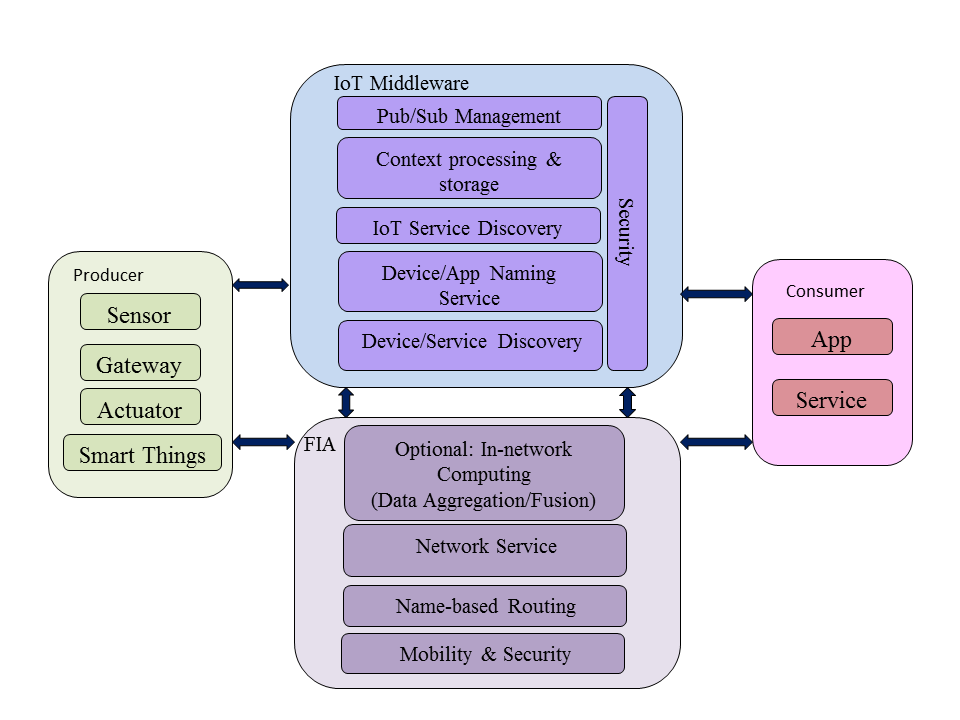
\includegraphics[width=\columnwidth]{figure/middleware_architecture.png}
\caption{\label{fig:mid_arch} ICN-IoT middleware functionality break down.}
\end{figure}
\subsection{Name Data Networking (NDN)}
NDN~\cite{zhang2014named} provides a receiver-driven architecture by transmitting two types of packets : Interest and Data. Consumer issues Interest of the hierarchical content name and forwards it to Data Producer. When the Interest arrives at some node (either intermediate router or Data producer) that owns the requested content, the node will reply the requested content along the reverse path to the Data Consumer.
NDN forwarding is supported by three data structures:
%NDN provides three types of key components to support such functionality.
Forwarding Information Base (FIB) maintains the forwarding information at each NDN node. The content prefix and out-face mapping is recorded in the FIB. Once a certain face receives Data packet for a pending Interest,  it could be added into the FIB to indicate a healthy data retrieving path. Pending Interest Table (PIT) is a data structure that maintains the set of pending Interest routed by the node expecting Data packet in return. PIT entry is created by receiving Interest,
%and filters the redundant Interest that carried the same content name.
Due to the limit size of PIT, every PIT entry is associated with a timeout which is defined or estimated by the consumer based on the round trip time. Once a matching Data packet is received, the NDN node forwards it through the face recorded in the PIT before this entry being removed. Content Store(CS) is a data cache for storing Data packet for matching Interest along the reverse path. In addition, due to the limit size of local CS, Data producer can define the freshness of the Data packet in order to timeout it in the CS. With such mechanism,
NDN decouples the content from its original location without location binding.

%NDN eliminates the notion of source and destination as it is in IP network, and handle routing only for Interest Packet.

\subsection{MobilityFirst (MF)}\label{sec:intro_mf}
MF~\cite{raychaudhuri2012mobilityfirst} utilizes GUID to name every network object, while separating this GUID from its actual network address. The separation of identifier(GUID) and its locator(network address)  allows MF to support dynamic address binding, multiple addressing binding and late binding. As shown as Figure ~\ref{fig:mf_arch}, MF core network architecture includes the following network components.

\vspace{1mm}\noindent{\bf Global Name Resolution Service(GNRS)}: GNRS is a centralized service that maintains mappings between GUID and network address. MF routers create the entries by performing an $Insert$ for the GUIDs of attached network devices and the associated network address, and query GNRS for a translation from GUID to the latest binding network address. Recent work shows that this translation performance is much better (50-100 ms delay) than DNS resolution~\cite{vu2012dmap}.

\vspace{1mm}\noindent{\bf Hybrid GUID/NA address routing}: Each MF router can make routing decision based on NA or GUID in the header of data packet, since routing decision are made by a hop-by-hop manner~\cite{nelson2011gstar}.

\vspace{1mm}\noindent{\bf Delay-Tolerant Network(DTN)}: Each MF router is able to cache data packets in its storage.
%The storage in each MF router provides the capability of caching the data packet.
By doing this,  data can be stored or forwarded depending on different routing policies, such as quality of the link which is  useful over wireless interface.
\begin{figure}
\centering
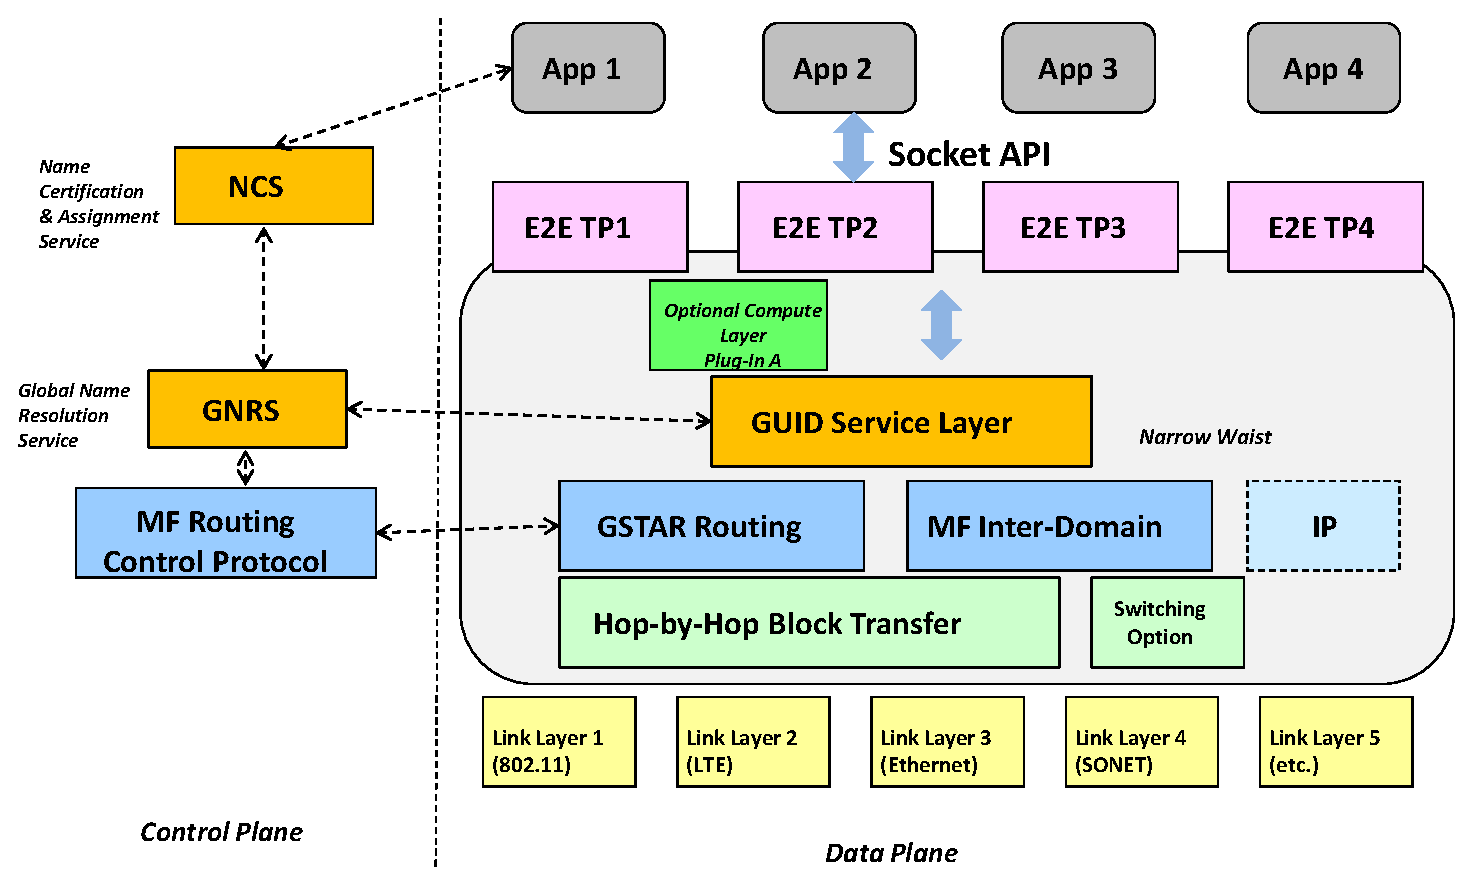
\includegraphics[width=\columnwidth]{figure/mf_arch.eps}
\caption{\label{fig:mf_arch}Mobilityfirst architecture.}
\end{figure}
%\subsection{MF Multicast}\label{sec:multi}

\vspace{1mm}\noindent{\bf MF multicast}: MF multicast is based on the idea of group GUID that gathers multiple network objects into one entity. Group GUID  to object GUID mapping is a one-to-many mapping that being maintained at GNRS server. Network object can claim to join the multicast group, and either edge router or a centralized management service will perform insertion of the object GUID to group GUID mapping to into GNRS server. When the first router queries GNRS server for a group GUID mapping, GNRS server returns a list of member GUIDs. The router assembles these GUIDs into the header and performs "Longest Common Path(LCP)" algorithm to determine the next hop address.Shown as Figure~\ref{fig:multicast}, routers look up the routing table for these GUIDs, and check if there are multiple next hops. When the number of the results is more than one, the router reassembles the header and forwards the copied packet to corresponding interfaces. If the number of multicast group members becomes significant, another approach can be adopted to resolve this issue--instead of assembling all GUIDs into the header after one query, each router on the path queries GNRS server for the group members and performs LCP to decide next hop.
\begin{figure}
\centering
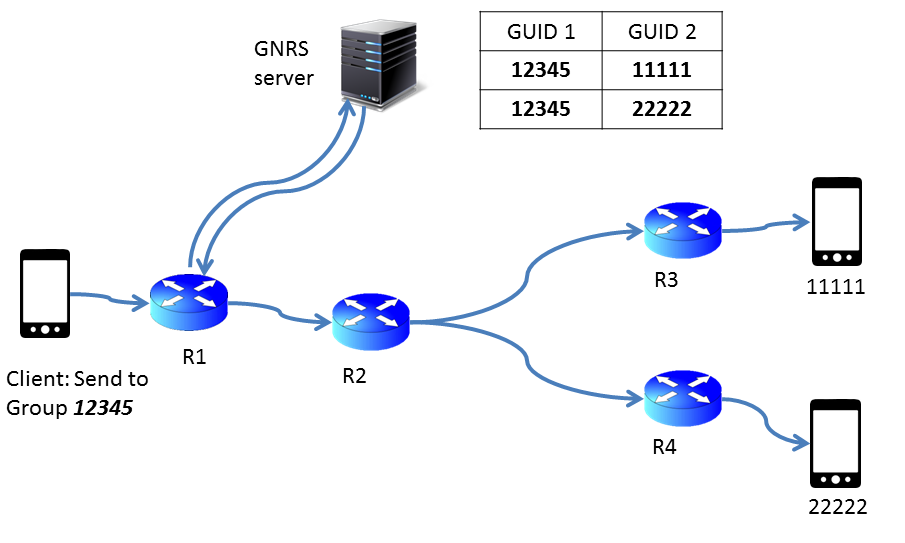
\includegraphics[width=\columnwidth]{figure/multicast.png}
\caption{\label{fig:multicast}MF multicast example: A client sends a message to Group 12345}
\end{figure}

\section{Related Work}
\label{sec:related}
ICN is a promising architecture for a general purpose future Internet, including Internet of Things. Previous works by Zhang Y. et al~\cite{zhang2013icn} and Li S. et al~\cite{compare_study} states the benefits that ICN network is capable to bring to IoT, including efficient data retrieval, well support of mobility, naming, scalability and security.

Some early work have demonstrated the feasibility of ICN on particular IoT system for both public space and home automation.  


Study by Amadeo et al.~\cite{amadeo2014multi} provides a solution on efficient multi-source data retrieval. It proposes a method to use one Interest to retrieve multiple data with different suffixes on different location by adjusting the traditional NDN protocol to support "prefix-based" interest. For example, a subscriber is interested in the resource named "/office/temperature", which is the information from multiple sensor deployed in his office. At the same time, temperature sensors should advertise their resource with this prefix and their own suffix(e.g sensor in the conference room should be named "/office/temperature/conferenceroom"). Hence, the subscriber can issue single interest to retrieve multiple resource.


George et al.~\cite{polyzos2015building} propose a Publish-Subscribe Internetworking ICN architecture
that identifier can be used to represent a thing, an application, a group of similar, or any contextual specific entity in the network. A Rendezvous Node functions as a middle box where advertisement from publisher and subscription request from subscriber can meet up to form a membership. 

Many study take one step further to implement IoT system over ICN architecture. In the study by Shang et al.~\cite{shang2014securing}, a practical use case that integrates NDN with Building Management System (BMS) is represented. It shows that human-readable hierarchical naming scheme brings convenience in configuring and managing large number of BACnet devices. Baccelli et al.~\cite{baccelli2014information} report a CCN experiment over a life-size IoT system. They port light-weight CCN-lite code with the RIOT operating system. Based on this platform, performance of various routing protocol and impact of caching have been measured.  


\section{ICN-IoT Middleware System Design}
In this section, we present the overall IoT middleware system design which consists of three distributed physical components, as shown in Figure~\ref{fig:phy}-- Aggregator, Local Service Gateway, and IoT server, and is composed of  four principle functionalities, including device discovery, device naming service, IoT service discovery and Pub/Sub management. 
%to develop IoT middleware over ICN network. 
In contrast to centralized or overlay functionality implementation in the legay IP-based IoT platform, our ICN-IoT middleware architecture pushes these functionalities down to the distributed compoents that not only can form a self-configurating subsystem to provide local service but also can act as a complete system to achieve global communcation. 
%In legacy IP-based IoT platform, these functionalities are almost implemented on a centralized server, or over-lay application. In our ICN-IoT middleware architecture, they are pushed down to distributed components which can form a self-configuring subsystem to provide local service as well as a complete system that enables global communication. 
\begin{figure}
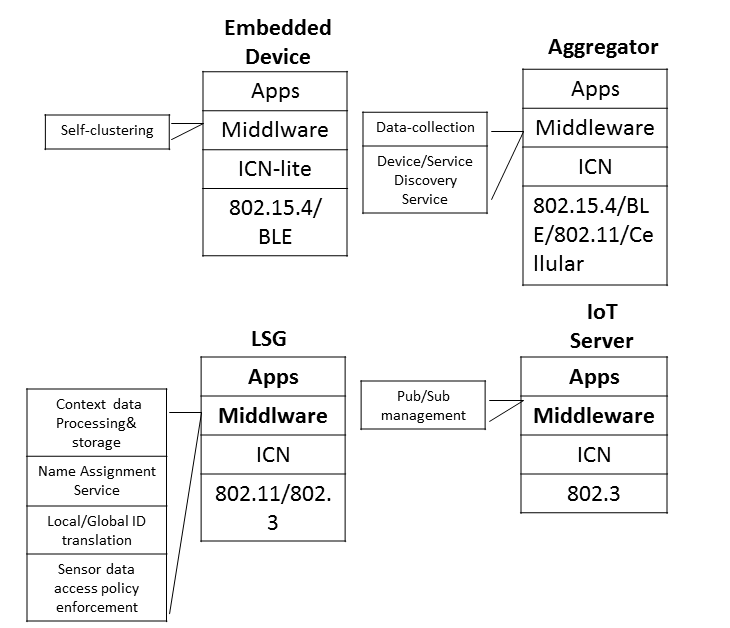
\includegraphics[width=\columnwidth]{figure/physical_comp.png}
\caption{\label{fig:phy}Physical components of ICN-IoT middleware}
\end{figure}
\subsection{Physical Components}\label{sec:physical}
\begin{itemize}
%\vspace{-2pt}
\item{\em Aggregator}:
It is the base-line component in our middlware architecture that interconnects various IoT service in the local network. An Aggregator usually plays two roles: one is to act as the gateway to bridge the communcation between other devices and resource-contraint wireless sensore and the other one is to integrate sensing/actuating service. 

%for resource-constraint wireless sensors, or it can be a device that integrates sensing/actuating service. 

%\vspace{-2pt}
\item{\em Local Service Gateway (LSG)}:
It connects local IoT system to the outside world, handes local name assignment and enforces  data access policy for local IoT devices. In addition, it can run context data processing service to publish only the information abstraction to IoT server.
%It connects local IoT system to the outside world. It handles local name assignment and sensor data access policy enforcement. Furthermore, context data processing service can be implemented within this entity to publish only the information abstraction to IoT server.    

%\vspace{-2pt}
\item{\em IoT Server}:
It is a centralized server that maintains subscription membership and provides lookup service for the subscribers. Unlike legacy IoT server that involves in the data path from publisher to subscriber, raising the concern of bandwidth of its interfaces being a bottleneck, IoT server in our architecture only involves in the control path where publishers and subscribers exchange their names and certificates.  

%Legacy IoT server also involves in the data path from publisher to subscriber, where the bandwidth of its interfaces could be a bottleneck. In contrast, IoT server in our architecture only involves in control path in which publishers and subscribers exchange their names and certificates.  
\end{itemize}

In the following subsections, we will discuss the breakdown functionality for each  physical component and demonstrate detail protocol design.

\subsection{Device Discovery}
The objective of device discovery is to contextually establish relationship for nodes in proximity and remote. Device discovery is a key component of any IoT system, and can be considerably simplified by the ICN network. In today's IoT systems, IP overlay device discovery module focuses on not only the reach-ability of a device, but also the device physical properties \cite{iotivity,alljoyn}. Moreover, a translation service is required to maintain the mapping from network addresses to physical attributes and manual configuration is necessary. ICN-IoT  device discovery, however,  does not involve any manual configuration or name traslation because ICN uses names to discover new devices. In what follows, we explain the ICN-IoT device discovery  in detail, including both devices that are able to run  full-stack protocols (referred to as \emph{resource-rich sensors}) and devices that are unable to do so (referred to as \emph{resource-constrained sensors}).

\vspace{1mm}\noindent{\bf Resource-rich sensors}: Many resource-rich sensors come with manufacture secure ID and model name, which need to be exposed to both the aggregator and LSG to facilitate device discovery. This aim can be achieved by different ways with respect to NDN and MF.  In NDN, this process is initiated by the configuration service running on LSG, which periodically broadcasts discovery Interests (using the name $/iot/model$). The new sensor replies to the discovery interest with its information, and the configuration service then registers the sensor and generates a local ICN name for the sensor. In MF, we can set the model number, $group$-$GUID$ as the destination address, and configuration service issues the request via multicasting. When receiving such request, the new device replies with the manufacture secure ID, and the configuration service registers the device and  generates a local ICN name to it.


\vspace{1mm}\noindent{\bf Resource-constrained sensors}: Many resource-constrained sensors connect to the Internet using the IEEE 802.15.4 technology via a border router~\cite{hui2008ip}. These sensors voluntarily discover each other in proximity and establish forwarding paths to the border router through self-organizing into a mesh network. Similarly, for our ICN-IoT middleware,  Aggregator acts as a border router, and neighbor discovery among sensors can be achieved differently with respect to NDN and MF as follows. In NDN, when a new sensor arrives, it broadcasts a neighbor discovery message to connect with neighbors. After establishing connectivity with neighboring sensors, it broadcasts an Interest named $/ndn/aggregatorservice$ to discover the Aggregator. In MF, neighbor discovery is naturally supported, and the new sensor simply needs to send a discovery request to a well-known broadcast GUID to discover the Aggregator. %On receiving, the destination Aggregator receives the request and registers the new device if there is matched service name.
The above process is shown as Figure~\ref{fig:device_dis} 
%\footnote{This figure is for either NDN or MF, or both?  The similar question for Figure 6}.
\begin{figure}
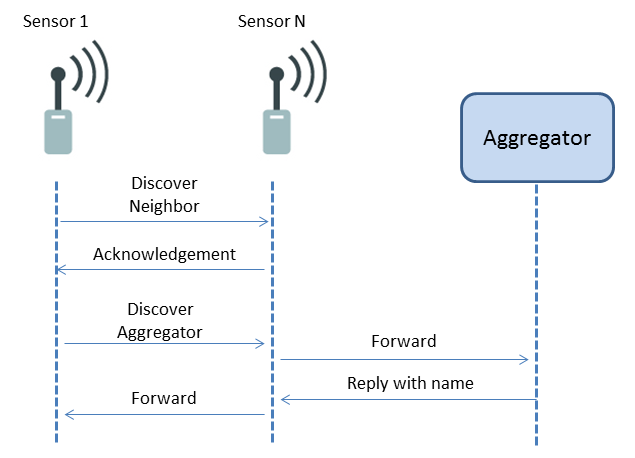
\includegraphics[width=\columnwidth]{figure/device_discovery.png}
\caption{\label{fig:device_dis}Device discovery for resource-constrained sensor}
\end{figure}



\subsection{IoT Service Discovery}

IoT services can be generally categorized into two classes: sensing and actuating. In today's IoT platforms, sensors are connected via a server, which requires considerable development effort such as maintaining a local name to IP mapping. In ICN-IoT, IoT service discovery and configuration becomes more efficient. Specifically, we consider two service discovery modes: $peer$-$to$-$peer$ and $master$-$slave$.


\vspace{1mm}\noindent{\bf Peer-to-peer Service Discovery}: In this mode, we consider the scenario in which an aggregator (referred to as the source aggregator) tries to discover an IoT service provided by another peer aggregator (referred to as destination aggregator). In NDN, the source aggregator broadcasts an interest using the well-known name $/area/servicename/certificate$, which will eventually reach the destination aggregator. NDN's Interest/Data mechanisms allows only one response for each Interest send while discovery requires to learn multiple entities, hence efficient discovery is realized using exclusion via Selectors in the protocol or as an overlay protocol~\cite{ravindran2013information}. In MF, this is handled by multicast (discussed in Section~\ref{sec:intro_mf}) instead of flooding the entire local network. All sensors that provide relevant services can join the multicast group identified by a $Group$-$GUID$. After establishing the multicast group, the source aggregator sends a request containing the service name and certificate to the multicast group.The destination aggregator that hosts the service checks the certificate and registers the source Aggregator if there is a matched service. It replies with an acknowledgement containing its certificate to the source aggregator. The message flow is shown as Figure~\ref{fig:ser_dis}
\begin{figure}
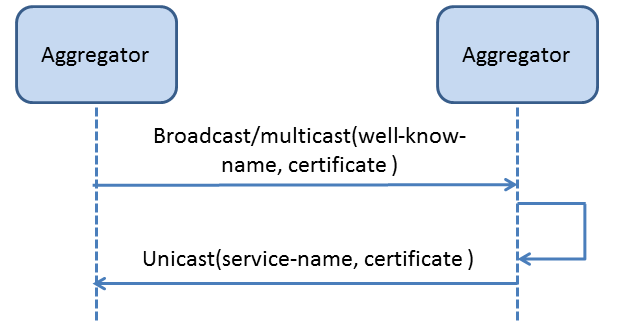
\includegraphics[width=\columnwidth]{figure/service_discovery.png}
\caption{\label{fig:ser_dis}Peer-to-peer service discovery}
\end{figure}
In an example of NDN smart home, a thermostat expresses a request to discover a AC service using well-known name $/home/ac/certificate$ via broadcast channel. In MF case, a multicast group GUID $1234$ can be assigned to all home appliance IoT service. The thermostat sends request containing the service name and certificate to $1234$. In both cases, the AC hosting this services replies with acknowledgement if all conditions match.

\vspace{1mm}\noindent{\bf Master-slave Service Discovery}: In some IoT applications, there are more than one sensing service or actuating service connecting to one control service. A source aggregator hosting control service expresses a request with service name and its certificate to discover a service from all  available aggregators. The destination aggregators verify the certificate. If valid, the destination aggregators register the source aggregator and  answer with acknowledgement containing their certificates if there is a matched service.

In the AC control NDN example, the number of AC service provider increases to three, which can be named as $/office/ac/1$, $/office/ac/2$ and $/office/ac/3$ . The thermostat expresses a partial name $/office/ac/certificate$ via a broadcast channel periodically. In the MF case, a multicast group GUID $1234$ can be assigned to identify AC service. The thermostat sends request with service name and certificate to $1234$. The destination ACs reply with their certificate if the request meets all criteria.

\subsection{Secure Device Discovery, Naming Service and Service Discovery}
Security guarantee is always treated as an essential function for the IoT middleware. Generally speaking, the security objective is to assure that the device that connects to the network should be authenticated, the provided services are authenticated and the data generated (through sensing or actuating) by both devices and services can be authenticated and kept privacy (if needed). To be specific, we consider the approach to secure device discovery, naming service and service discovery, because other services, such as pub/sub management and context processing \& storage, can be properly secured according to application-specific demands.
 
Recall that our goal is to assure that either device or service itself is authenticated, attemptting to prevent sybil (or spoofing) attack \cite{sybil} and the assigned name is closely binding to the device (or service). In what follows, let us consider how to secure device discovery and name assignment. Suppose that the device (i.e., sensor) can be either programmable so that before deployment the owner can preload some identity information (such as secure ID, a pair of public/private key and a certificate) , or has some manufacture ID and a pair of public/private key (which is certified by the manufacturer). That is, the device is associated with information including device identity, public/private keys ($PK_{device}, SK_{device}$) and a certificate either from the owner or the manufacturer which certifies the device identity and public/private keys. For the ICN-IoT middleware on top of NDN, when discovering a device, the aggregator will first verify the device identity (e.g., the device can generate a signature with the private key $SK_{device}$ and present the signature and the certificate to the aggregator so that the aggregator can verify it), and then assign a name to the device as follows: the aggregator will issues a request to LSG together with its device identity and $PK_{device}$, so that LSG can assign an ICN name and generate a certificate (certifying the binding of ICN name, $PK_{device}$). To this end, the ICN name and the certificate will be sent back to the aggregator and will be stored locally if the device is resource-restricted. Otherwise, the ICN name and the certificate will be passed to the device. For the MF-IoT, assigning a network name (GUID) for a device is rather straightforward: after verifying the device identity, the Aggregator
%generates a pair of public/private key ($PK_{mf}, SK_{mf}$), and
inserts the public key $PK_{device}$ and device information to the upper layer component to verify if there is a conflict in the corresponding scope. Specifically, LSG is in charge of local scope and IoT server guarantees the global uniqueness. Finally, the unique public key is used a GUID for the new device. Analogously, service discovery can be secured in a similar way.
 
Note that the above discussion assumes that there exists public key infrastructure (a centralized and hierarchical system) , which greatly simplify the system trust model. In some ad hoc network this assumption may not hold and some other trust mechanisms may need to be employed, such as PGP. Moreover, in order to comply with the capability of resourced-restricted devices, light-weight cryptographic primitive (such as symmetric cryptography) may be used instead of public key cryptography.

%\subsection{Secured Device Naming Service}
%A key step towards realizing a unified IoT platform is the ability to assign names that are unique within the scope and lifetime of each device, data items generated by these devices, or a group of devices towards a common objective. Naming service is usually triggered by device discovery. For NDN architecture, automatic naming scheme is following the hierarchical manor with minimum assumption -- device is always named after its attached point's name, and every physical component in our ICN-IoT middleware should have at least one name. Figure~\ref{} illustrates how a new device can be named using ICN-IoT middleware on top of NDN architecture. A sensor is being discovered by a nearby Aggregator. This Aggregator generate a key pair issues a request to the LSG with its manufacture ID and public key. On receiving of the request, the LSG generates a certificate and an ICN name for the new sensor, then send back to the Aggregator. Last, the Aggregator forward the information to the sensor or store it if the sensor has limited resource. In MF, generating a GUID for a new sensor is rather straightforward: the nearby Aggregator generates a key pair for the sensor, and inserts the public key and device information to the upper layer component to verify if there is a conflict in the corresponding scope. Specifically, LSG is in charge of local scope and IoT server guarantees the global uniqueness.Finally, the unique public key is used a GUID for the new device.

\subsection{Publish/Subscribe Management}
Data Publish/Subscribe (Pub/Sub) is an important function for ICN-IoT, and is responsible for resource sharing and management. In conventional IP network, most of the IoT platforms provide a centralized server to aggregate all IoT service and data. While 
%resource is published as service,  
this centralized architecture ensures the availability, but it poorly supports scalability and high bandwidth consumption due to high volume of control and data exchange. Thus, we consider a decentralized pub/sub model in ICN-IoT middleware. Specifically, we will discuss rendezvous mode and a data-control separated mode.

\vspace{1mm}\noindent{\bf Rendezvous Mode}: Rendezvous mode is a classical pub/sub scheme in which data and request meet at an intermediate node. While NDN is a Pull-based architecture without supporting the Pub/Sub mode naturally,  COPSS~\cite{chen2011copss} proposes a solution to fix this problem. It integrates a push based multicast feature with the pull based NDN architecture at the network layer by introducing Rendezvous Node(RN). RN is a logical entity that resides in NDN. The publisher first forwards a Content Descriptor (CD) as a snapshot to the RN. RN maintains a subscription table, and receives the Subscription message from subscriber. The data publisher just sends the content using Publish packet by looking up FIB instead of PIT. If the same content prefix is requested by multiple subscribers, RN will deliver one copy  of content downstream, which reduces the bandwidth consumption substatially.

\begin{figure}
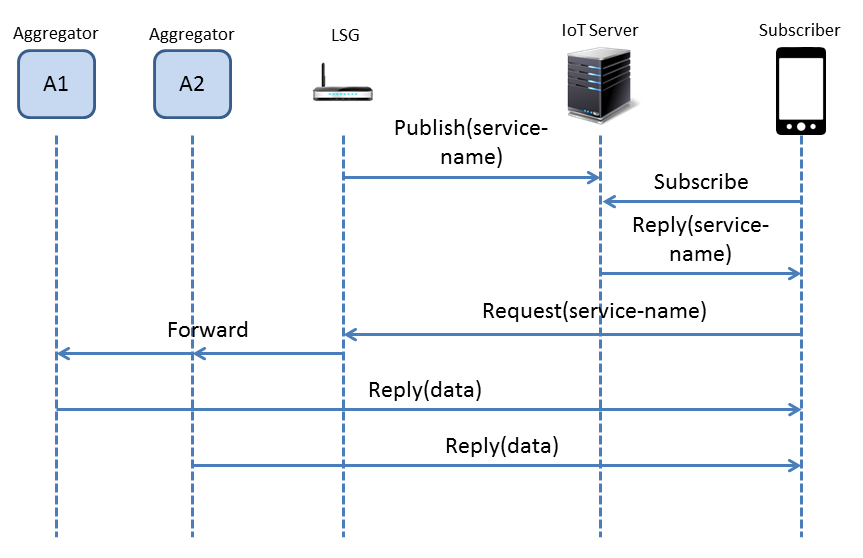
\includegraphics[width=\columnwidth]{figure/pub_sub.png}
\caption{\label{fig:pubsub}Publish/subscriber management message flow}
\end{figure}
\vspace{1mm}\noindent{\bf Data-control separated Mode}:Compared with Rendezvous mode in which data plane and control plane both reside on the same ICN network layer, we consider an architecture where the control message is handled by the centralized server while data is handled by ICN network layer.  Following the naming process mentioned above, the LSG has the ICN name for the local resource which is available for publishing on IoT server.  IoT server maintains the subscription membership, and receives subscription requests from subscribers. Since the subscribers has non knowlege about the number of resource providers and their identities  in a dynamic scenario,  IoT server has to take responsibility of grouping and assigning group name for the resource. The generic message flow for publish/subscribe function is shown in Figure~\ref{fig:pubsub}, and we will illustrate the detail in each individual architecture.
In NDN, the grouping resource is intuitive : all resource have the same schematic prefix will be grouped together, and the prefix can be used to identify the service. The traditional NDN dose not support using a common partial name to retrieve multiple resource, but M. Amadeo et al. ~\cite{amadeo2014multi} provides a solution to resolve this issue by introducing long-life multi-source Interest in PIT.
MF takes advantage of  $Group$-$GUID$ to identify a service provided by multiple resources. This $Group$-$GUID$ will be distributed to the subscriber as well as the publisher. In an example of NDN,  it uses the common prefix$/home/monitoring/$ to identify a group of resource that provides multiple monitoring services such as $/home/monitoring/temperature$ and $/home/monitoring/light$. The subscriber retrieves the prefix from the IoT server, and sends Interest toward the resource. In a MF example, $GUID$-$x$ identifies the "home monitoring" service that combines with "light status" and "temperature". The resource producers, i.e. the host of "temperature" and the host of "light status" are notified that their services belong to $GUID$-$x$, then listen on $GUID$-$x$. The subscriber sends the request containing  $GUID$-$x$ through multicasting which ultimately reach the producers at the last common node. Once receiving the request, the resource producer unicasts the data to the subscriber. In addition, if multiple resource consumers subscribe to the same resource, the idea of $Group$-$GUID$ can be reused here to group the consumers to further save bandwidth using multicast.


\section{Evaluation}
In this section, we investigate the efficiency of service discovery based on MF multicast, MF unicast and NDN interest selector. We have conducted a detailed experiment in NS3-based MF simulator and ndnSIM.  MF network protocol is implemented over standard NS3 P2P module and the experiments are running in a tree-based topology. In MF multicast case, $Group GUID$ is used to identify a service at unknown location, i.e., service host (SH) can be at any leaves of the tree while service requester (SR) attaches to the root of the tree. SR issues a request and the first router then performs  GNRS lookup for the $Group GUID$. On receiving of the service request message, the matched receivers will reply with a acknowledgement to the service requester via unicast. While in MF unicast case, we configures the SR to issue request periodically and each matched SH will reply the request sequentially.In NDN selector experiment,  SR expresses Interest with name "/service", and corresponding full name is "/service/\\{1,2,..., n\}". On receiving of the response from one of the SHs, the SR appends the response's name to the exclusion list of a Interest and re-express a Interest with the same name. This operation will repeat until no response comes back. Figure~\ref{fig:5_service_over} shows the overhead in terms of total message per service discovery in a 5-tier tree. We observe that MF multicast introduces the least overhead among three schemes, as it triggers only one GNRS lookup per request, and the routers only forwards request duplicates based on the next common hop(s). When the number of  SH increases to 5, NDN interest selector and MF unicast achieve similar performance. This is due to selector prevents  both routers and SHs forwarding the discovered responses, which decreases the total response message. In MF unicast, total message number grows linearly as the number of SH increases. Figure~\ref{fig:6_service_over} demonstrates the result of the same experiment in a 6-tier tree. NDN selector scheme encounters the highest overhead due to the impact of network scale increment on Interest broadcast. 
     
\begin{figure}
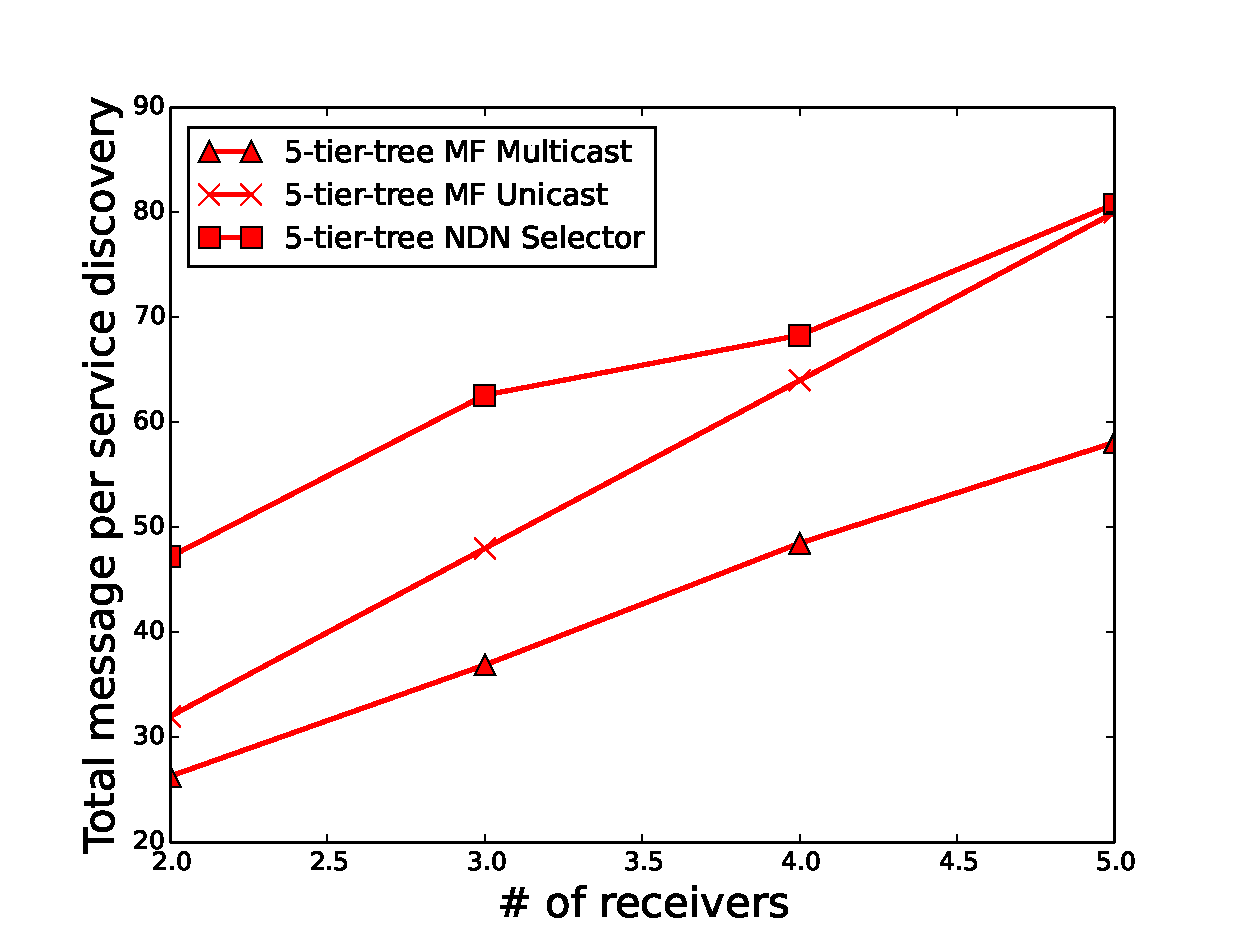
\includegraphics[width=\columnwidth]{figure/5_service_discovery_overhead.eps}
\caption{\label{fig:5_service_over}Overhead of service discovery in 5-tier tree}
\end{figure}

\begin{figure}
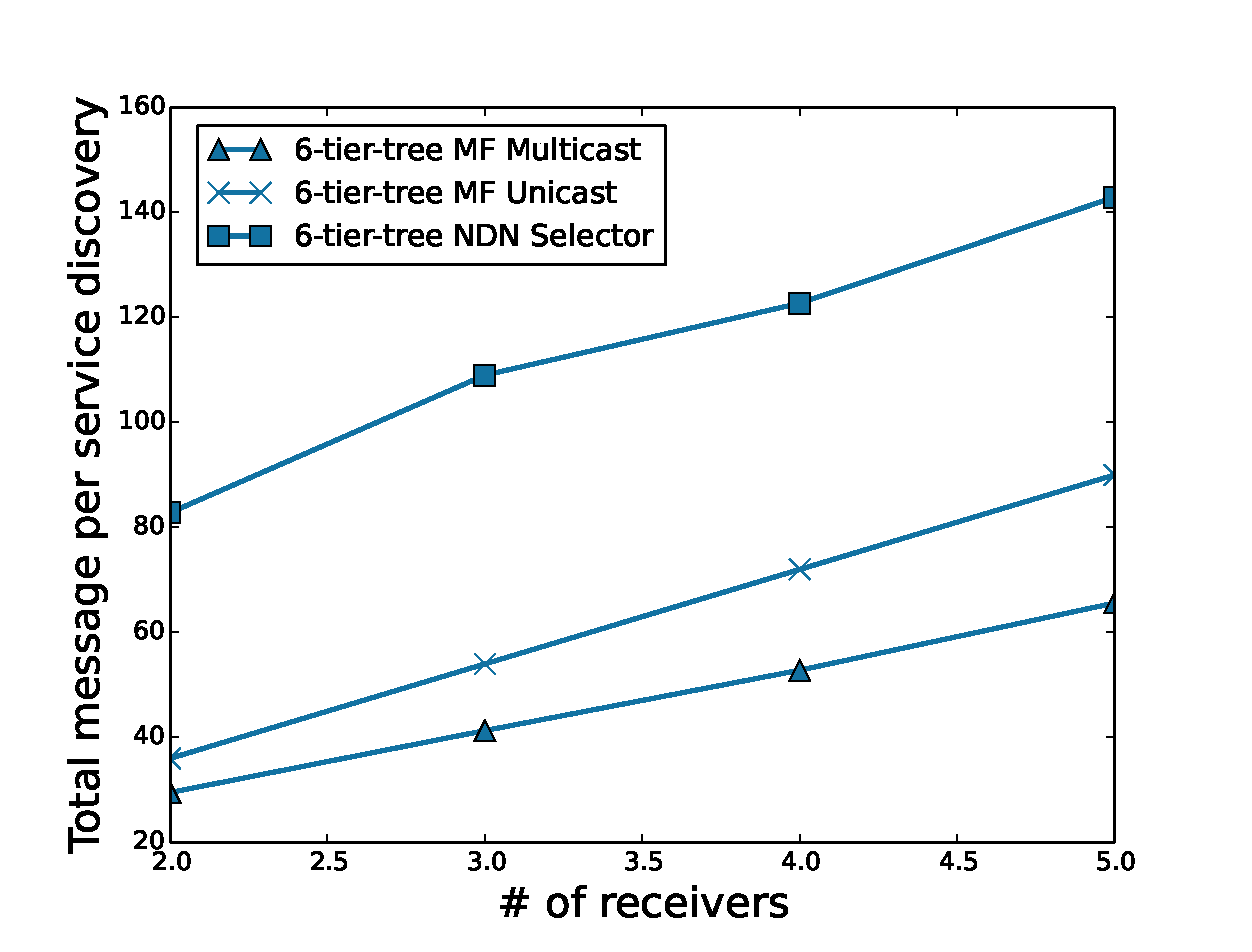
\includegraphics[width=\columnwidth]{figure/6_service_discovery_overhead.eps}
\caption{\label{fig:6_service_over}Overhead of service discovery in 6-tier tree}
\end{figure}
%\subsection{Service Discovery}
%\subsection{Multi-source Retrieval}


\section{Conclusion}
Conclusion
%\balance
%\scriptsize
%\footnotesize
%\small
\bibliographystyle{sig-alternate-10pt}
\bibliography{iot}
\end{document}